% Umlaufzeit eines Satelliten in Abhängigkeit von der Bahnhöhe
% Benötigt: pgfplots, tikz


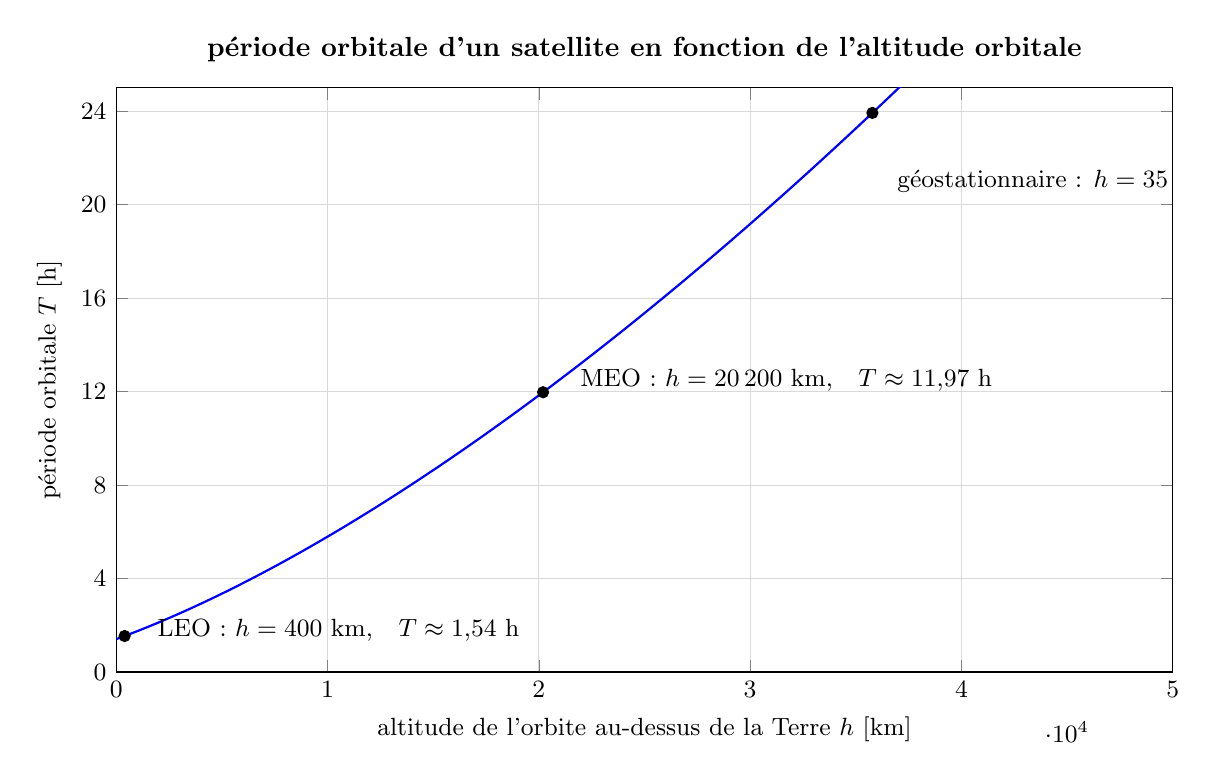
\begin{tikzpicture}
\begin{axis}[
    width=15cm,
    height=9cm,
    xlabel={altitude de l’orbite au-dessus de la Terre $h$ [km]},
    ylabel={période orbitale $T$ [h]},
    xmin=0, xmax=50000,
    ymin=0, ymax=25,
    xtick={0,10000,20000,30000,40000,50000},
    ytick={0,4,8,12,16,20,24},
    grid=both,
    minor grid style={gray!15},
    major grid style={gray!30},
    tick label style={font=\small},
    label style={font=\small},
    title={période orbitale d’un satellite en fonction de l’altitude orbitale},
    title style={font=\bfseries},
]

% T = 2*pi*sqrt((R_E+h)^3/mu)
% R_E = 6371 km
% mu = 398600.4418 km^3/s^2
\addplot[
    domain=0:50000,
    samples=300,
    thick,
    blue
]
{2*pi*sqrt((6371+x)^3/398600.4418)/3600};

% LEO : 400 km
\addplot[only marks, mark=*, mark size=2pt]
coordinates {(400,{2*pi*sqrt((6371+400)^3/398600.4418)/3600})};

\node[anchor=west, font=\small] at
(axis cs:1500,1.8)
{LEO : $h=400$ km,\quad $T\approx1{,}54$ h};

% MEO : GPS altitude 20200 km
\addplot[only marks, mark=*, mark size=2pt]
coordinates {(20200,{2*pi*sqrt((6371+20200)^3/398600.4418)/3600})};

\node[anchor=west, font=\small] at
(axis cs:21500,12.5)
{MEO : $h=20\,200$ km,\quad $T\approx11{,}97$ h};

% Geostationary orbit
\addplot[only marks, mark=*, mark size=2pt]
coordinates {(35786,{2*pi*sqrt((6371+35786)^3/398600.4418)/3600})};

\node[anchor=west, font=\small] at
(axis cs:36500,21.0)
{géostationnaire : $h=35\,786$ km,\quad $T\approx23{,}93$ h};

\end{axis}
\end{tikzpicture}

